\section{Results}

Before the behaviour of the algorithms is analysed, some plots of kinematic variables are shown
in figure~\ref{fig:kinematics}.
It can be seen that the algorithms do not greatly differ on the kinematics of the events.
In particular, \spectral{} does not appear to sculpt any distributions.

\begin{figure}[htp]
    \begin{minipage}[c]{0.7\textwidth}
    \begin{center}
    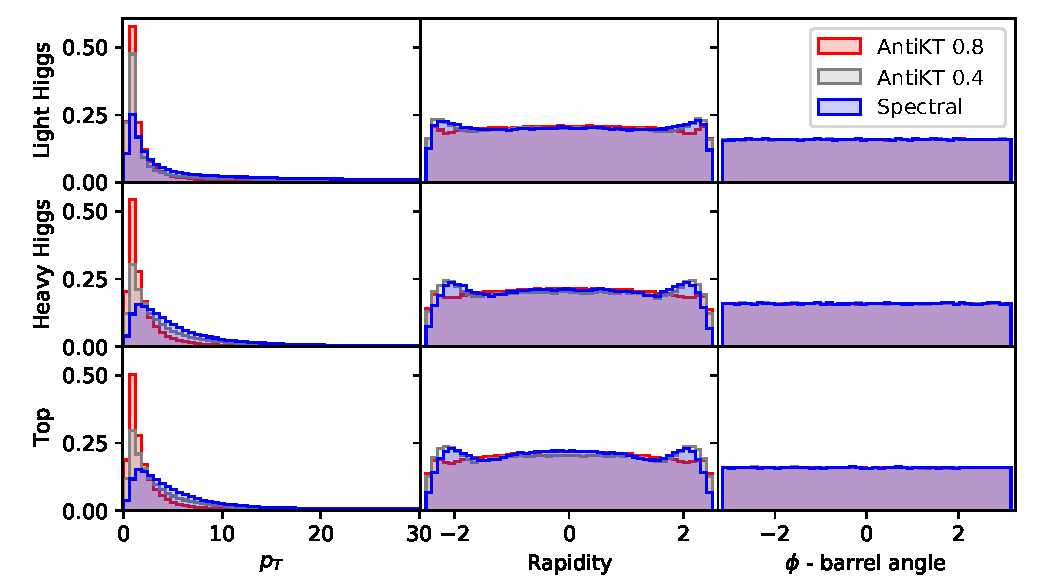
\includegraphics[width=\textwidth]{graphics/kinematics}
\end{center}
\end{minipage}
    \begin{minipage}[c]{0.25\textwidth}
        \caption{Basic kinematic variables for each of the datasets and three clustering algorithms.
            In the first column it can be seen that there is some difference in the typical mass produced.
            In the second column the rapidity shows some edge effects,
            the algorithms cluster jets at the edge of the barrel slightly differently.
            In the final column the barrel angle show no noticeable changes.
        }\label{fig:kinematics}
\end{minipage}
\end{figure}

\subsection{Infrared-collinear safety}
Shape variable spectra would be sensitive to IRC divergences.
For each configuration of the clustering algorithm we expect an IRC safe algorithm to give the 
same shape variable spectrum for both LO and NLO datasets.
Changes in the shape variables indicate sensitivity to the soft and collinear radiation that
has been included at NLO.
This comparison is made in figure~\ref{fig:IRC_singles2}.
It can be seen in this figure that little difference exists between \genkt{} and \spectral{}.


\begin{figure}[htp]
    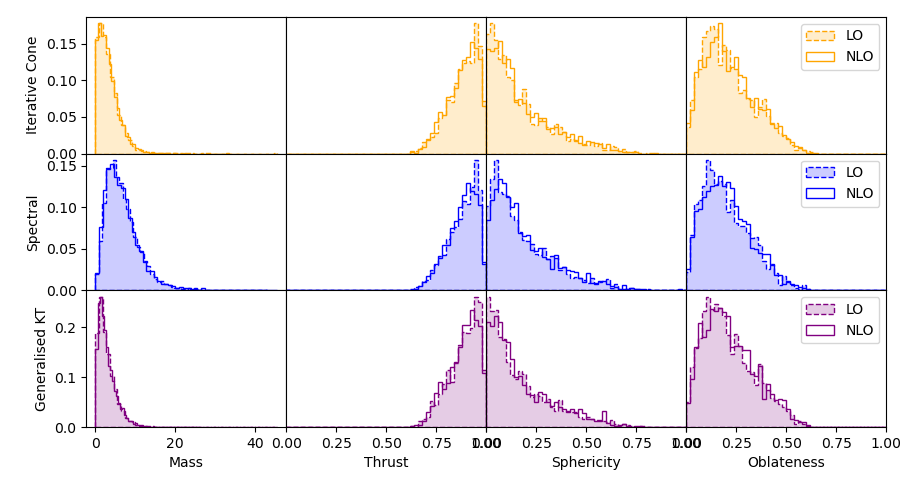
\includegraphics[width=\textwidth]{graphics/IRC_singles2}
    \caption{Spectrums for jet properties created with LO and NLO datasets.
             The \(4\) jets with highest \(p_T\) from each event are used to 
             form these plots.
             The columns from left to right are; the jet mass, 
             thrust of the jets, sphere city of the jets and oblateness of the jets.
             the barrel angle of the jets and the rapidity of the jets.
             Algorithms where configured (i.e. settings of \stoppingdeltar{} chosen)
             to give sensible results on
             this dataset, therefore may not represent worst case scenarios.
             Looking at these graphs it is not immediately clear that the \genkt{}
             algorithm is IRC safe and the Iterative Cone algorithm is unsafe, 
         much less what the status of Spectral clustering is.}\label{fig:IRC_singles2}
%    \begin{minipage}[c]{0.47\textwidth}
%        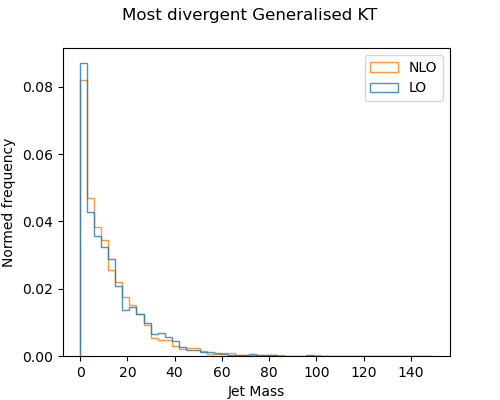
\includegraphics[width=\textwidth]{graphics/worst_antikt_histOnly.png}
         %        \caption{The jet mass spectrums of the \genkt{} algorithms that
%                 differed the most between LO and NLO datasets.
%                 This algorithm had a \(p_T\) exponent of \(1.\),
%                 (so the form of the \(p_T\) factor is between Cambridge-Aachen and KT),
%                 it used taxi-cab distances in physical space
%                 and \(\stoppingdeltar{} = 1.5\).
%                 Little divergence can be seen.
%        }
%    \end{minipage}\hfill
%    \begin{minipage}[c]{0.45\textwidth}
%        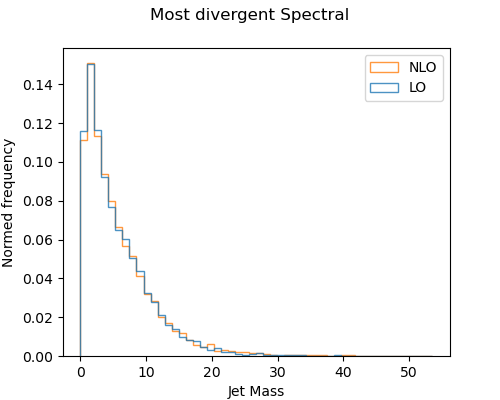
\includegraphics[width=\textwidth]{graphics/worst_spectral_histOnly.png}
%        \caption{The jet mass spectrums of the Spectral algorithms that
%                 differed the most between LO and NLO datasets.
%                 This algorithm calculated affinities as
%                 \(a_{i,j} = \text{exp}\left((\delta \phi_{i, j}^2 + \delta y_{i, j}^2)/0.3\right)\).
%                 The Laplacian is symmetric and 
%                 as many eigenvector as can be found are used which are
%                 normalised as \(x_{i,\text{normed}} = x_i/\lambda_i^{1.8}\).
%                 There is no use of \(p_T\) and \(\stoppingdeltar{} = 1.3\).
%                 Little divergence can be seen.
%        }\label{fig:spectralircexample}
%    \end{minipage}
%    \begin{minipage}[c]{0.48\textwidth}
%        \includegraphics[width=\textwidth]{graphics/worst_iterativecone_histonly.png}
%        \caption{The jet mass spectrums of the Iterative Cone algorithms that
%                 differed the most between LO and NLO datasets.
%                 This algorithm had a \(p_T\) exponent of \(1.\),
%                 (so the form of the \(p_T\) factor is between Cambridge-Aachen and KT),
%                 it used taxi-cab distances in physical space
%                 and \(\stoppingdeltar{} = 0.34\).
%                 Some divergence is seen, particularly at low mass.
%        }\label{fig:iterconeircexample}
%    \end{minipage}
\end{figure}    

%
%\begin{figure}[htp]
%    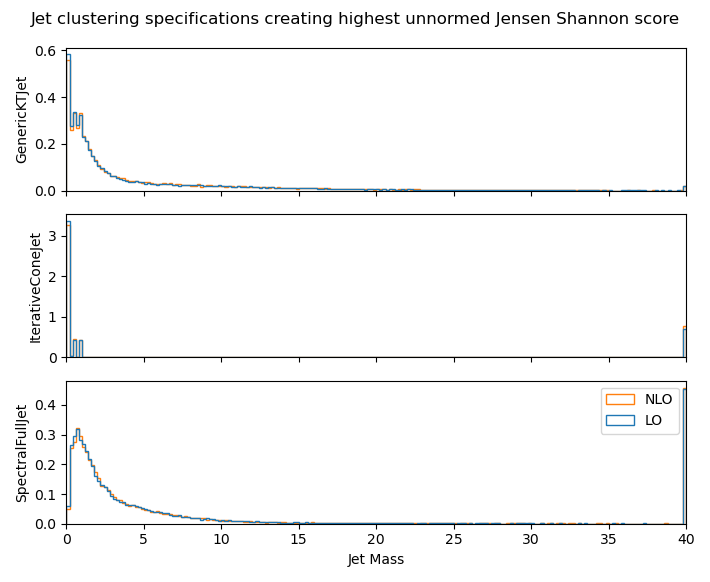
\includegraphics[width=1.\textwidth]{graphics/same_bin_size_worst_all_jets.png}
%    \caption{Same plots as previous, but with the same x-axis.
%        Last bin is overflow bin.
%    }
%\end{figure}    
%
However, this method of establishing IRC safety only looks at one hyperparameter configuration and could be accused to cherry-picking.
As described in section~\ref{sec:IRCmethod} this can be systematically compared for many hyperparameter configurations by calculating a Jensen-Shannon
score for each LO-NLO pair of jet mass spectrums.
If the Jensen-Shannon metric is low, then the two distributions are similar and appear IRC safe.
To further clarify the result we include an algorithm known to be IRC unsafe, the \itercone{} algorithm.
This can be seen in fig~\ref{fig:unnormedJS}.

\begin{figure}[htp]
    \begin{minipage}[c]{0.6\textwidth}
    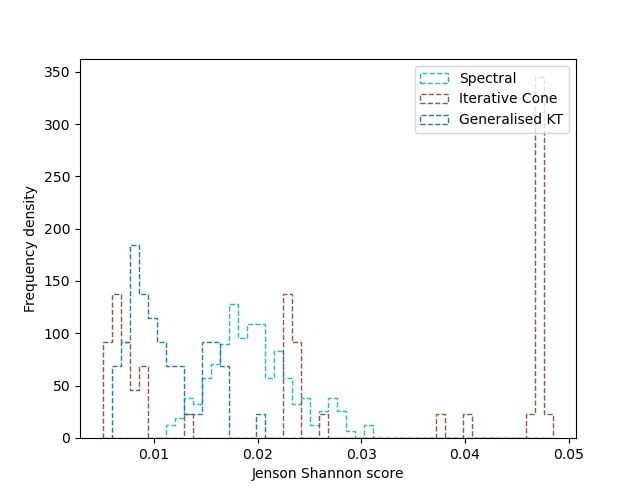
\includegraphics[width=1.\textwidth]{graphics/JensenShannon_unnormed.png}
    \end{minipage}\hfill
    \begin{minipage}[c]{0.35\textwidth}
    \caption{Here is the raw distribution of Jensen-Shannon scores.
        Each count is a Jenson Shannon score between a probability density of jet mass from LO data and
        from NLO data, as described in section~\ref{sec:IRCmethod}.
        Counts at low values indicate insensitivity to IRC difference between the LO and NLO data,
        thus IRC safety.
        Spectral methods produce Jensen Shannon scores similar to \genkt{}
        methods. Only Iterative cone produced high Jenson shannon scores indicating changes
        between the LO and NLO spectrums.
     }\label{fig:unnormedJS}
    \end{minipage}
\end{figure}    

This comparison is slightly complicated by the fact that we must use a completely different set of events,
so if a clustering algorithm tends to produce more noisy mass spectrums (on varied events)
anyway it will increase the gap between the NLO and the LO datasets even if no IRC sensitivity is present.
Again, as described in section~\ref{sec:IRCmethod} the influence of this noise can be investigated.
This can be seen in fig~\ref{fig:jensenshannon}.

From both these figures it is clear that \spectral{} is IRC safe.
The change in jet mass spectrum between an LO and NLO dataset is consistently small,
resulting in small Jensen Shannon scores,
across a representative range of parameter configurations.
This contrasts with \itercone{}, for which the jet mass spectra at LO and NLO 
differ significantly, resulting in large Jensen Shannon scores, for many configurations.
This is not unexpected, as the inputs to \spectral{}
are the same as for the Cambridge-Aachen algorithm, 
which is itself IRC safe.
However it is good to have a verification in data.

\begin{figure}[htp]
    \begin{minipage}[c]{0.6\textwidth}
    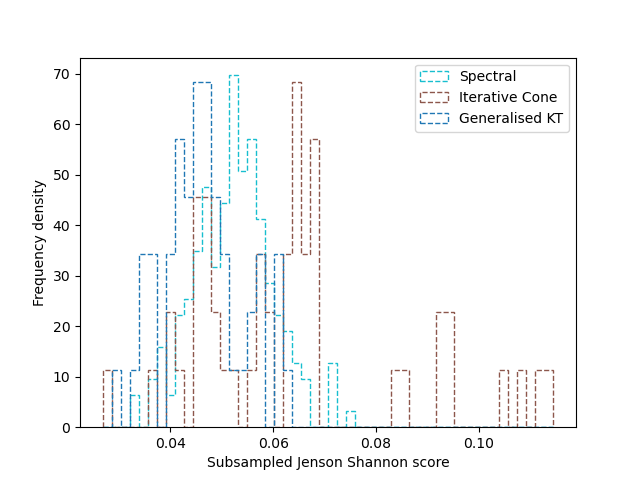
\includegraphics[width=1.\textwidth]{graphics/JensenShannon.png}
    \end{minipage}\hfill
    \begin{minipage}[c]{0.35\textwidth}
    \caption{Here is the distribution of subsampled Jensen-Shannon scores.
        Each count is a subsampled Jenson Shannon score between a probability density of jet mass from LO data and
        from NLO data, as described in section~\ref{sec:IRCmethod}.
        Counts at low values indicate insensitivity to IRC difference between the LO and NLO data,
        thus IRC safety.
        Spectral methods produce Jensen Shannon scores similar to \genkt{}
        methods. Only Iterative cone produced high Jenson shannon scores indicating changes
        between the LO and NLO spectrums.
        From this it is clear that \spectral{} methods are IRC safe,
        and that the volume of data used to produce this figure and figure~\ref{fig:unnormedJS},
        was sufficient to mitigate the effects of noise.
    }\label{fig:jensenshannon}
    \end{minipage}
\end{figure}    

\FloatBarrier{}
\subsection{Mass peak reconstruction}
In this section \antikt{} algorithms, with jet radius \(\ktstoppingdeltar{} = 0.4\) and \(\ktstoppingdeltar{} = 0.8\)
are compared to the \spectral{} algorithm specified in section~\ref{sec:spectralmethodparam}.

The jets are tagged using MC truth.
Each of the \bthing{quarks} created by a signal particle (such as a light higgs)
tag the closest jet (by angle, \(\sqrt{(y_i - y_j)^2 + (\phi_i - \phi_j)^2}\)) provided that jet is no further than \(0.8\) away.
From this point on, only jets tagged this way are considered.


Firstly, jet multiplicities, that is number of tagged jets found per event are given.
These can be seen for three data samples described in section~\ref{sec:particle_data} in fig~\ref{fig:multiplicity}.


\begin{figure}[htp]
    \begin{center}
        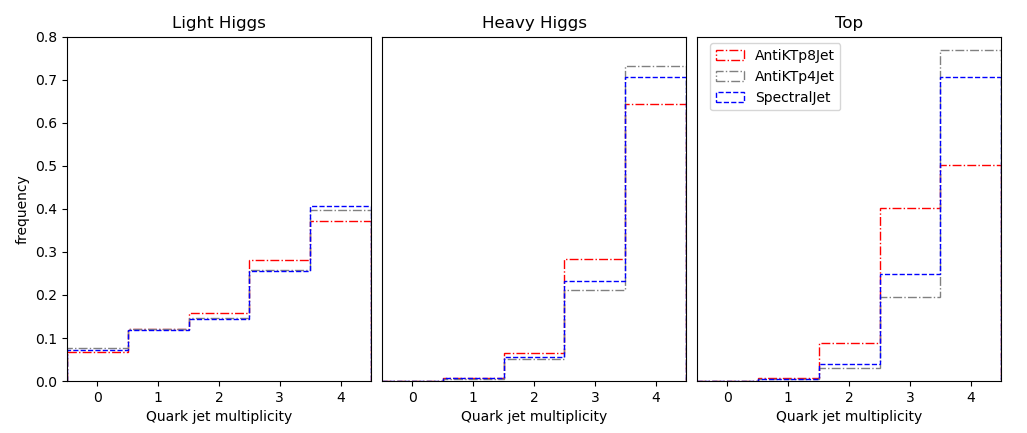
\includegraphics[width=0.7\textwidth]{graphics/multiplicity/all3.png}
    \end{center}
    \caption{Jet multiplicities for \spectral{}, on three data samples described in section~\ref{sec:particle_data}.
        It is seen that \spectral{} produces the best multiplicity for light higgs events.
        For the heavy higgs and top datasets 
        \spectral{} creates a multiplicity closer to that of \antikt{} with \(\ktstoppingdeltar{} = 0.4\) 
        than \(\ktstoppingdeltar{} = 0.8\).
    }\label{fig:multiplicity}
\end{figure}    



%As the data is simulated, it is possible to compare the performance of clustering algorithms to Monte Carlo truth.
%Each higgs cascade event contains 4 \bthing{quarks} and for each of them it is possible to identify the particle into which they decayed, as a subset of the particles in the final state.
%Henceforth the detectable decay products of the \bthing{quark} will be called the descendants of the \bthing{quark}.
%For two reasons it is not possible for this clustering algorithm to gather all the descendants
%of each \bthing{quark} into one jet:
%firstly, not all the descendants make the \(p_T\) and \(\eta\) cuts, so some are discarded before clustering;
%secondly, the descendants of the \bthing{quarks} in an event are not mutually exclusive, due to interactions during hadronisation the quarks share descendants, and our clustering algorithm does produce exclusive clusters.
%
%Combining these factors with the \(p_T\) cuts, almost \(2/3\) of the objects could be reconstructed in theory.

%Knowing the parts of the final state that are descended from each \bthing{quark} creates a clear
%allocation of jets to quarks.
%For each quark, the jet that contains the greatest mass in descendent particles is tagged to represent that quark.

Mass peaks are constructed from the tagged jets.
Again, \antikt{} with \(\stoppingdeltar{}_\text{kt} = 0.8, 0.4\) is given for comparison.
In figure~\ref{fig:best_correct_h_allocation} three selections are plotted; firstly only events where jets for all 4 \bthing{quarks} is found
are plotted, reconstructing the mass of the SM Higgs.
Each event also contains two light higgs.
These are differentiated by the mass of the particles they generate that pass particle cuts,
in effect they are ranked by how well they were picked up by the detector.
The light higgs with more mass visible to the detector is called the better observed light higgs,
the light higgs with less mass visible in the detector is called the less observed light higgs.
Two jets are required to reconstruct a light higgs.
The correct jets for each Higgs reconstruction are identified using MC truth,
so the correct pairings are always made.
If two jets are not found the event is not included.

It can be seen that Spectral clustering forms the sharpest peaks, and peaks at the correct mass.


\begin{figure}[htp]
    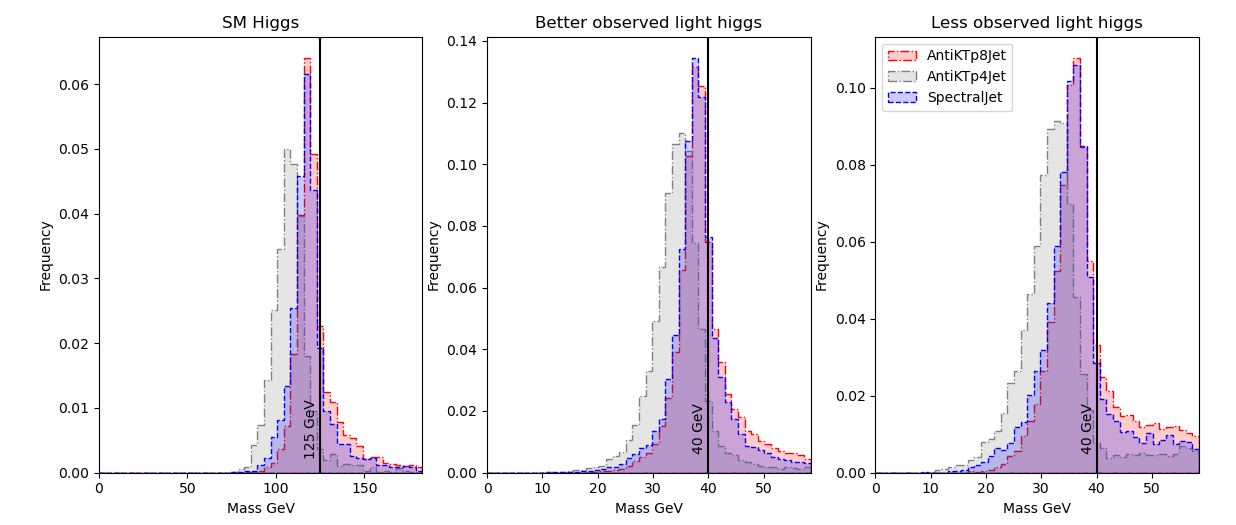
\includegraphics[width=1.\textwidth]{graphics/mass_peaks/light_long_correct_frequency.png}
    \caption{
Three selections are plotted; firstly only events where jets for all 4 \bthing{quarks} is found
are plotted, reconstructing the mass of the SM Higgs.
Then the two light Higgs in each event are differentiated by the mass of their descendants,
in effect they are ranked by how well they were picked up by the detector.
The light higgs with more mass visible to the detector is called the better observed light higgs,
the light higgs with less mass visible in the detector is called the less observed light higgs.
    }\label{fig:best_correct_h_allocation}
\end{figure}    

Figure~\ref{fig:heavy_correct_mass_peaks} the exercise is repeated for the heavy higgs dataset.
All the parameters of \spectral{} are the same as for for light higgs dataset,
so the algorithm is being used on a dataset for which it was not tuned.
The performance is still excellent, with sharp peaks at the correct masses.
Note that, in figure~\ref{fig:multiplicity},
it was seen that spectral clustering achieved better multiplicity than \antikt{} \(\ktstoppingdeltar{} = 0.8\) on this dataset.
While the multiplicity of \antikt{} \(\ktstoppingdeltar{} = 0.4\) is a little better, the location of the peak for
\(\ktstoppingdeltar = 0.4\) is wrong.

\begin{figure}[htp]
    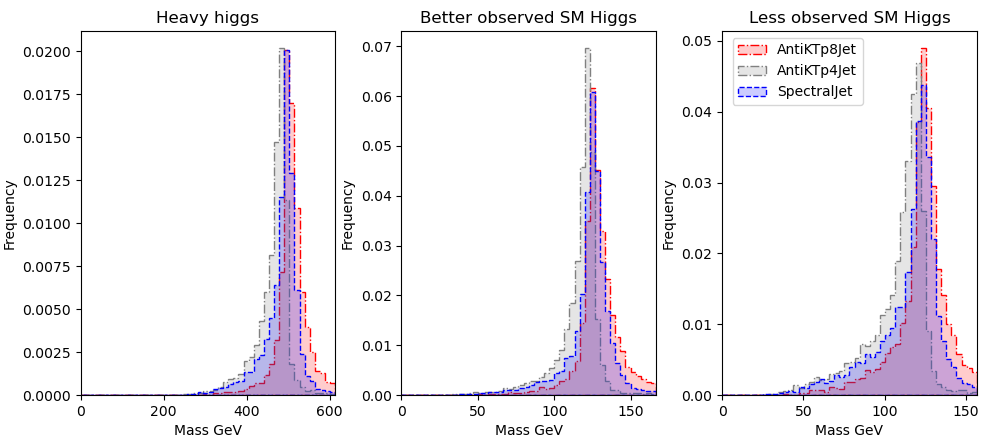
\includegraphics[width=1.\textwidth]{graphics/mass_peaks/heavy_long_correct_frequency.png}
    \caption{
Three selections are plotted; firstly only events where jets for all 4 \bthing{quarks} is found
are plotted, reconstructing the mass of the heavy higgs.
Then the two SM Higgs in each event are differentiated by the mass of their descendants,
in effect they are ranked by how well they were picked up by the detector.
The SM Higgs with more mass visible to the detector is called the better observed SM Higgs,
the SM Higgs with less mass visible in the detector is called the less observed SM Higgs.
}\label{fig:heavy_correct_mass_peaks}
\end{figure}    


\begin{figure}[htp]
    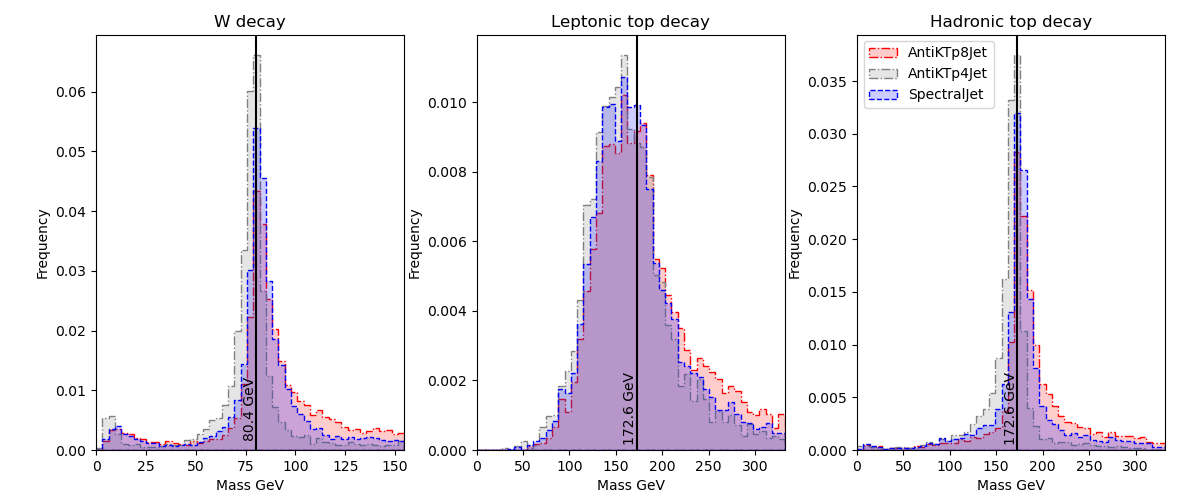
\includegraphics[width=1.\textwidth]{graphics/mass_peaks/top_long_correct_frequency.png}
    \caption{
        Three selections are plotted; firstly just the mass of the jet or jets that reconstruct the hadronic \(W\) is plotted.
        Then the reconstructed mass of the leptonic top is plotted,
        this depends on one reconstructed \bthing{jet} and then a missing \(p_T\) reconstruction
        for the leptonic \(W\).
        Finally, the mass of the hadronic top is plotted, as reconstructed from the 
        \(W\) jets and the \bthing{jet} from the top.
    }\label{fig:top_correct_mass_peaks}
\end{figure}    

Finally, in figure~\ref{fig:top_correct_mass_peaks} the mass peaks for the semileptonic top decay are shown.
Three reconstructions are given; the hadronic \(W\) is reconstructed.
This may be the mass of one jet which has been tagged by both the quarks from the \(W\),
of the mass of two separate jets tagged by the quarks from the \(W\).
If either of the quarks from the \(W\) failed to tag a jet the event is not used to reconstruct the \(W\).
The mass of the hadronic top is then reconstructed in events where the hadronic \(W\) could be reconstructed and the \bthing{jet}
from the hadronic top is also found.
The leptonic top is then reconstructed in events where \bthing{jet} from the top is found.
The leptonic reconstruction uses the momentum of the electron and missing momentum (from unseen final state particles)
to reconstruct the leptonic \(W\), and only proceeds if a real mass is obtained.

It can be seen here that \spectral{} is adapting to jets of a different radius.
While before its behaviour had most resembled \(\ktstoppingdeltar{} = 0.8\)
it has now moved closer to \(\ktstoppingdeltar{} = 0.4\).
Semileptonic top events would typically be processed using \(ktstoppingdeltar{} = 0.4\).
The peaks of \spectral{} are not quite as narrow as \(\ktstoppingdeltar{} = 0.4\),
but they improve on \(\ktstoppingdeltar{} = 0.8\) and the location is correct.

%\begin{figure}[htp]
%    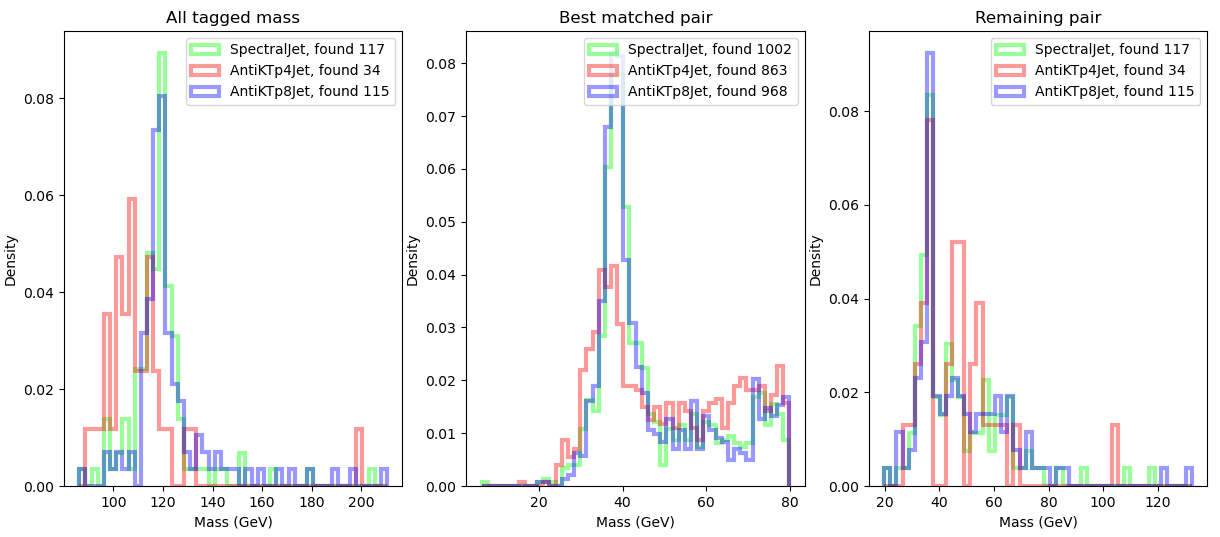
\includegraphics[width=1.\textwidth]{graphics/show2_40.png}
%    \caption{Mass peaks for the light higgs cascade;
%    \(p^+ p^+ \rightarrow H_{125\text{GeV}} \rightarrow h_{40\text{GeV}} h_{40\text{GeV}} \rightarrow \beau \bbar \beau \bbar\).
%        Jets are required to have at least 2 particles and \(15\) GeV \(p_T\).
%        The left hand peak is the mass of all jets in events where 4 jets are reconstructed.
%        The central plot is the mass of the dijet pair closest to \(40\) GeV,
%        the right hand plot is the remaining dijet pair.
%    }
%\end{figure}    
%
%\begin{figure}[htp]
%    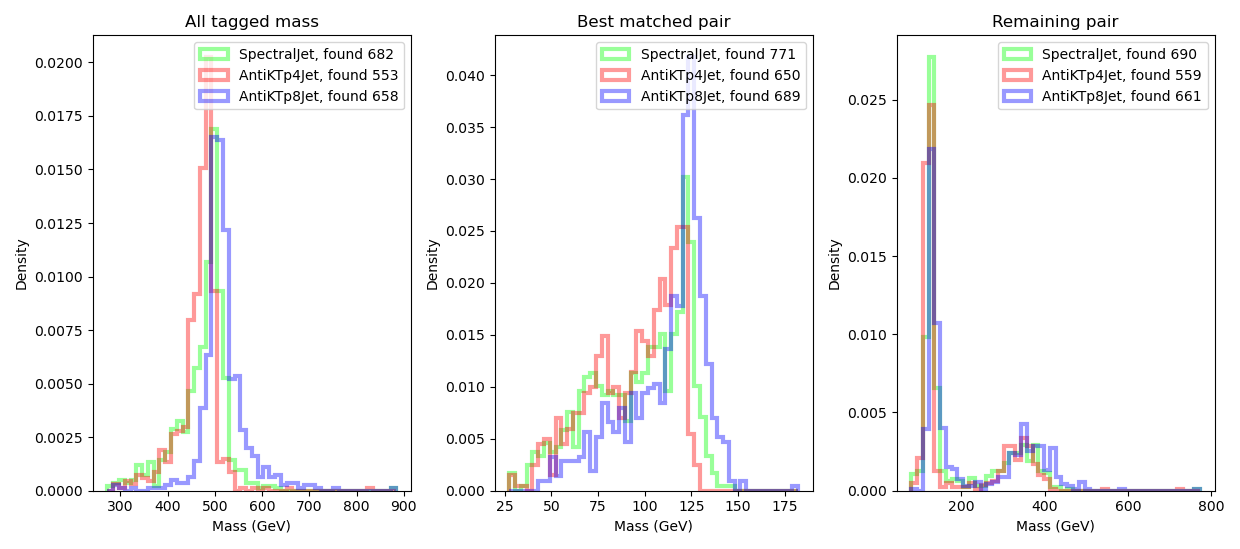
\includegraphics[width=1.\textwidth]{graphics/show2_125.png}
%    \caption{Mass peaks for the heavy higgs cascade,
%    \(p^+ p^+ \rightarrow H_{500\text{GeV}} \rightarrow h_{120\text{GeV}} h_{120\text{GeV}} \rightarrow \beau \bbar \beau \bbar\).
%        Jets are required to have at least 2 particles and \(30\) GeV \(p_T\).
%        The left hand peak is the mass of all jets in events where 4 jets are reconstructed.
%        The central plot is the mass of the dijet pair closest to \(125\) GeV,
%        the right hand plot is the remaining dijet pair.
%    }
%\end{figure}    



%There are also some values that can be given to compare these two jets;
%\begin{enumerate}
%    \item Quality fraction~\cite{JetQuality2008}. A window on the reconstructed masses,
%        size proportional to the root of mass of the object to be reconstructed,
%        across the data. The total number of generated objects (in this dataset 2000)
%        is divided by the maximum number of reconstructed objects in the window,
%        and this is the quality width.
%        
%        \[\text{\antikt{} (\(\stoppingdeltar{} = 0.8\)) Quality Fraction} = 1.33\text{GeV}\]
%        \[\text{Spectral Quality Fraction} = 1.33\text{GeV}\]
%    \item Quality width~\cite{JetQuality2008}. A required fraction of the generated objects,
%        in this case \(0.15\) is selected.
%        The smallest mass window that can capture this fraction is determined.
%        
%        \[\text{\antikt{} (\(\stoppingdeltar{} = 0.8\)) Quality Width} = 0.00141\text{GeV}\]
%        \[\text{Spectral Quality Width} = 0.000129\text{GeV}\]
%    \item Signal mass lost. The mass of the particles descendent from the light higgs
%        that are visible on the barrel is compared to the mass of the subset of those
%        particles that was found in the jet. The higher the number the more
%        signal particles are missing from the jet.
%        \[\text{\antikt{} (\(\stoppingdeltar{} = 0.8\)) Signal mass lost} = 1.80\text{GeV}\]
%        \[\text{Spectral Signal mass lost} = 2.17\text{GeV}\]
%    \item Background contamination. The mass of all the background objects,
%        either from the wrong higgs or from gluons, found in jets.
%        The higher the number the more the jets are tending to include too many particles.
%        \[\text{\antikt{} (\(\stoppingdeltar{} = 0.8\)) Background contamination} = 1.92\text{GeV}\]
%        \[\text{Spectral Background contamination} = 1.56\text{GeV}\]
%\end{enumerate}
%
